%% UNCOMMENT FOR SLIDES
\documentclass[table]{beamer}
\mode<presentation>

%% UNCOMMENT FOR HANDOUTS
%\documentclass[handout]{beamer}
\usepackage{handoutWithNotes}
\pgfpagesuselayout{2 on 1}[a4paper,border shrink=5mm]
%\pgfpagesuselayout{4 on 1 with notes}[a4paper,border shrink=5mm]
%% GENERIC STYLE SETTINGS BELOW
\usetheme{default}
\usepackage{listings}
\usepackage{multirow}
\usepackage{xcolor}

\usebackgroundtemplate{

\includegraphics[width=\paperwidth,height=\paperheight]{images/hutton_background}
}
%% PRESENTATION CONFIGURATION PARAMETERS %%%%%%%%%%%%%%%%%%%%%%%%%%%%%%%%%%%%%%%
%\titlebackgroundfile{images/hutton_title}
%\framebackgroundfile{images/hutton_background}
\definecolor{hutton_green}{HTML}{78A22F}
\definecolor{hutton_purple}{HTML}{872175}
\definecolor{hutton_blue}{HTML}{569BBE}
\usefonttheme{structurebold}
\setbeamercolor{alerted text}{fg=orange}
\setbeamercolor{background canvas}{bg=white}
\setbeamercolor{block title}{bg=hutton_purple}
\setbeamercolor{frametitle}{fg=hutton_purple}
\setbeamercolor{title}{fg=black}
\setbeamercolor{titlelike}{fg=hutton_green}
\setbeamercolor{author}{fg=hutton_purple}
\setbeamercolor{author in head/foot}{fg=white}
\setbeamercolor{title in head/foot}{fg=white}
\setbeamercolor{section in head/foot}{fg=hutton_purple}
\setbeamercolor{normal text}{fg=black}
\setbeamercolor{frametitle}{fg=hutton_purple}
\setbeamerfont{block title}{size={}}
\setbeamerfont{author}{size=\footnotesize}
\setbeamerfont{date}{size=\footnotesize}
\setbeamercolor{section in toc shaded}{fg=hutton_purple}
\setbeamercolor{section in toc}{fg=hutton_purple}
\setbeamercolor{subsection in toc shaded}{fg=hutton_purple}
\setbeamercolor{subsection in toc}{fg=hutton_purple}
\setbeamertemplate{itemize item}[circle]
\setbeamertemplate{itemize subitem}[circle]
\setbeamertemplate{itemize subsubitem}[circle]
\setbeamertemplate{itemize subsubsubitem}[circle]
\setbeamercolor{itemize item}{fg=hutton_purple}
\setbeamercolor{itemize subitem}{fg=hutton_purple}
\setbeamercolor{itemize subsubitem}{fg=hutton_purple}
\setbeamercolor{itemize subsubsubitem}{fg=hutton_purple}
\setbeamercolor{enumerate item}{fg=hutton_purple}
\setbeamercolor{enumerate subitem}{fg=hutton_purple}
\setbeamercolor{enumerate subsubitem}{fg=hutton_purple}
\setbeamercolor{enumerate subsubsubitem}{fg=hutton_purple}
\setbeamercolor{alerted text}{fg=hutton_green}
\setbeamerfont{alerted text}{series=\bfseries}
% This command makes that acrobat reader doesn't changes the colors of the slide
% when there are figures with transparencies.
\pdfpageattr {/Group << /S /Transparency /I true /CS /DeviceRGB>>}

%Disables discrete bottom navigation bar
%\beamertemplatenavigationsymbolsempty

%Mess about with the slide titles to avoid the corner images,
\setbeamertemplate{frametitle}
{
\vspace{0.05\textheight}
\noindent\quad\begin{minipage}[t][0.12\textheight][t]{0.85\textwidth}
\insertframetitle\par
\end{minipage}
}

%Mess about with title page to avoid the big logo on right
\setbeamertemplate{title page}{
    \begin{picture}(0,0)
            %This ends up on top of the default background image, rather than replacing it:
            \put(-30,-165){%
                
\includegraphics[width=\paperwidth,height=\paperheight]{images/hutton_title}
            }
            \put(0,-75){%
                \begin{minipage}[b][0.4\textheight][t]{0.75\textwidth}
                    \usebeamerfont{title}\usebeamercolor[fg]{title}{\inserttitle\par}
                    \usebeamerfont{subtitle}\usebeamercolor[fg]{subtitle}{\insertsubtitle\par}
                \end{minipage}
            }
            \put(0,-135){%
                \begin{minipage}[b][0.1\textheight][t]{\textwidth}
                    \usebeamerfont{author}\usebeamercolor[fg]{author}{\insertauthor\par}
                \end{minipage}
            }
    \end{picture}
}

%%%%%%%%%%%%%%%%%%%%%%%%%%%%%%%%%%%%%%%%%%%%%%%%%%%%%%%%%%%%%%%%%%%%%%%%%%%%%%%%

% LISTINGS SETTING
% Settings for code listings in lstlistings

\lstset{ %
  backgroundcolor=\color{yellow},   % choose the background color; you must add \usepackage{color} or \usepackage{xcolor}
  basicstyle=\tiny\ttfamily,        % the size of the fonts that are used for the code
  breakatwhitespace=false,         % sets if automatic breaks should only happen at whitespace
  breaklines=true,                 % sets automatic line breaking
  captionpos=b,                    % sets the caption-position to bottom
  commentstyle=\color{red},    % comment style
  deletekeywords={...},            % if you want to delete keywords from the given language
  escapeinside={\%*}{*)},          % if you want to add LaTeX within your code
  extendedchars=true,              % lets you use non-ASCII characters; for 8-bits encodings only, does not work with UTF-8
  frame=single,                    % adds a frame around the code
  keepspaces=true,                 % keeps spaces in text, useful for keeping indentation of code (possibly needs columns=flexible)
  keywordstyle=\color{blue},       % keyword style
%  language=Octave,                 % the language of the code
  morekeywords={*,...},            % if you want to add more keywords to the set
  numbers=left,                    % where to put the line-numbers; possible values are (none, left, right)
  numbersep=5pt,                   % how far the line-numbers are from the code
  numberstyle=\tiny\color{gray}, % the style that is used for the line-numbers
  rulecolor=\color{black},         % if not set, the frame-color may be changed on line-breaks within not-black text (e.g. comments (green here))
  showspaces=false,                % show spaces everywhere adding particular underscores; it overrides 'showstringspaces'
  showstringspaces=false,          % underline spaces within strings only
  showtabs=false,                  % show tabs within strings adding particular underscores
  stepnumber=1,                    % the step between two line-numbers. If it's 1, each line will be numbered
  stringstyle=\color{violet},     % string literal style
  tabsize=4,                       % sets default tabsize to 2 spaces
  title=\lstname                   % show the filename of files included with \lstinputlisting; also try caption instead of title
}


%%%
% TITLE PREAMBLE
\title[Intro to Bioinformatics] % (optional, only for long titles)
{An Introduction to Bioinformatics Tools}
\subtitle{Part 2: BLAST}
\author[Pritchard, Cock] % (optional, for multiple authors)
{Leighton~Pritchard \and Peter~Cock}
\institute[The James Hutton Institute] % (optional)
{
  Information and Computational Sciences\\
  The James Hutton Institute
}
\date[May 2014] % (optional)
{Bioinformatics Training, 29$^{th}$, 30$^{th}$ May 2014}
\subject{Bioinformatics}

%%%
% TOC
% Show table of contents, with current section highlighted,
% at the start of each section

\AtBeginSection[]
{
  \begin{frame}
    \frametitle{Table of Contents}
    \tableofcontents[currentsection,hideallsubsections]
  \end{frame}
}

%%%
% START DOCUMENT
\begin{document}

\frame[plain]{\titlepage}

% Learning Outcomes
\section{Introduction}
\subsection{Introduction}
\begin{frame}
  \frametitle{Learning Outcomes}
  \begin{itemize}
    \item How BLAST searches work
    \item How the way BLAST searches work affects your results
    \item Why search parameters matter
    \item Setting search parameters
 \end{itemize}
\end{frame}    
  
\begin{frame}
  \frametitle{About Bioinformatics Tools}
  \begin{center}
    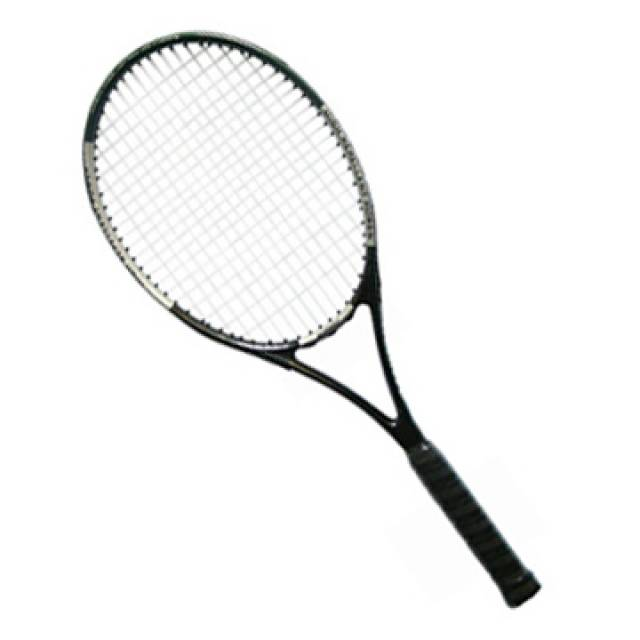
\includegraphics[width=0.5\textwidth]{images/racquet} 
    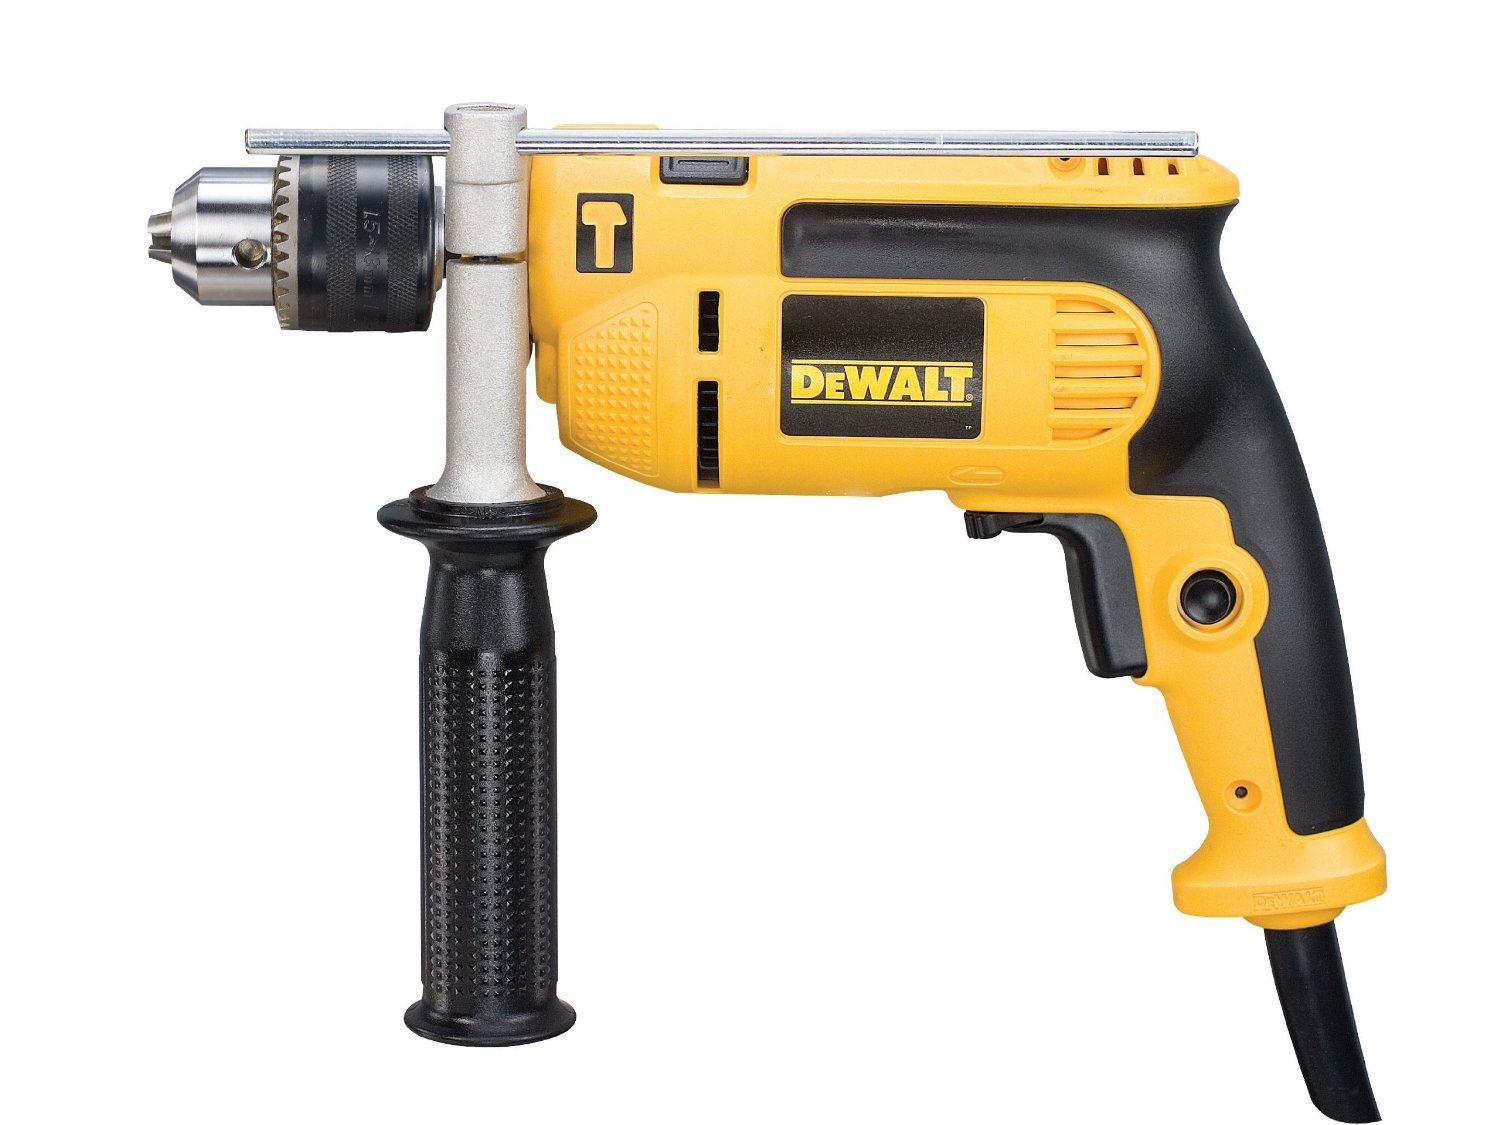
\includegraphics[width=0.5\textwidth]{images/drill}       
  \end{center}
\end{frame}      

\begin{frame}
  \frametitle{Why So Much Detail?}
  \begin{itemize}
    \item You're going to go away and do lots of BLAST searches
    \item Everyone uses BLAST - not everyone uses it well
    \item Easier to fix problems if you know how it works
    \item Understanding what's going on helps avoid misuse/abuse
    \item Understanding what's going on helps use the tool more effectively
    \item Not so much detail, really
    \begin{itemize}
      \item like knowing about $T_m$ and ion concentration effects, not molecular 
               orbitals or thermodynamics (but ask if you're interested ;) )
    \end{itemize}
  \end{itemize}
\end{frame}      

  
%%%
% SECTION: BLAST Essentials
% Sequence alignment in general
\section{Alignment} 
  % What is BLAST?
%
% Introductory slides illustrating in broad terms what BLAST is.
% The point here is to express that it's a search tool, not an alignment tool.

\subsection{What is BLAST?}
  \begin{frame}
  \frametitle{What BLAST Is}
  \begin{itemize}
    \item<1-> BLAST:
    \begin{itemize}
      \item<1-> Basic (it's actually sophisticated)
      \item<1-> Local Alignment (what it does: local sequence alignment)
      \item<1-> Search Tool (what it does: search against a database)
    \end{itemize}
    \item<2-> The most important software package in bioinformatics?
    \item<2-> Fast, robust, sequence similarity search tool
    \item<2-> Does not necessarily produce optimal alignments
    \item<2-> Not foolproof.
  \end{itemize}
\end{frame}
  
\begin{frame}
  \frametitle{What A BLAST Search Is}
  \begin{itemize}
    \item Every BLAST search is an \textit{in silico} hybridisation experiment
    \item BLAST search = identification of similar sequences in a database
    \item Results depend on:
    \begin{itemize}
      \item query sequence
      \item BLAST program (including version and BLAST vs BLAST+)
      \item database
      \item parameters
    \end{itemize}
  \end{itemize}
\end{frame}  
  % Sequence Alignment
%
% A brief, broad introduction to sequence alignment

\subsection{Sequence Alignment}
\begin{frame}
  \frametitle{Alignment Search Space}
  Consider two biological sequences to be aligned$\ldots$
  \begin{itemize}
    \item One sequence on the \textit{x}-axis, the other on the \textit{y}-axis
    \item Each point in space is a pairing of two letters
    \item Ungapped alignments are diagonal lines in the search space, gapped alignments have short ``breaks''
    \item There may be one or more ``optimal'' alignments
  \end{itemize}
  \begin{center}
    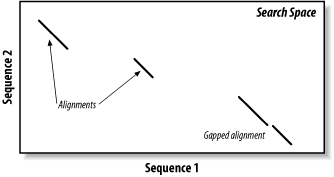
\includegraphics[width=0.4\textwidth]{images/search_space} 
  \end{center}
\end{frame}
    
\begin{frame}
  \frametitle{Global \textit{vs} Local Alignment}
  \begin{itemize}
    \item<1-> Global alignment: sequences are aligned along their entire lengths
    \item<1-> Local alignment: the best subsequence alignment is found
    \item<2-> Consider an alignment of the same gene from two distantly-related eukaryotes, where:
    \begin{itemize}
      \item<2-> Exons are conserved and small in relation to gene locus size
      \item<2-> Introns are not well-conserved but large in relation to gene locus size
    \end{itemize}
    \item<2-> Local alignment will align the conserved exon regions
    \item<2-> Global alignment will align the whole (mostly unrelated) locus
  \end{itemize}
 \end{frame}

  % Dynamic Programming
%
% A cartoon-like introduction to dynamic programming in sequence alignment.
% The aim is to illustrate the method, with some easy to parse examples, 
% emphasising that the method is general and mathematical, and that any 
% biology resides only in (i) the scoring scheme (substitution matrix) and (ii)
% the scientists' heads

\subsection{Dynamic Programming}
  \begin{frame}
  \frametitle{Our Goal}
  \begin{itemize}
    \item<1-> We aim to align the words
    \begin{itemize}
      \item<1-> \texttt{COELACANTH}
      \item<1-> \texttt{PELICAN}
    \end{itemize}
    \item<2-> Each identical letter (match) scores +1
    \item<2-> Each different letter (mismatch) scores -1
    \item<2-> Each gap scores -1
    \item<3-> \emph{Alignment is maximisation of the alignment score}
  \end{itemize}
\end{frame}   
   
\begin{frame}
  \frametitle{Initialise the matrix}
  \begin{center}
    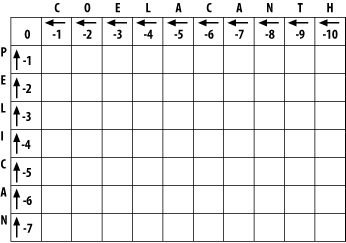
\includegraphics[width=0.65\textwidth]{images/initialise}
    \end{center}
\end{frame}   
   
\begin{frame}
  \frametitle{Fill the cells}
  \begin{center}
    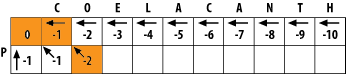
\includegraphics[width=0.65\textwidth]{images/fill_start} \\
    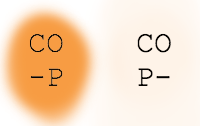
\includegraphics[width=0.3\textwidth]{images/fill_start_letters}
  \end{center}
\end{frame}     

\begin{frame}
  \frametitle{Fill the matrix -- represents all possible alignments \& scores}
  \begin{center}
    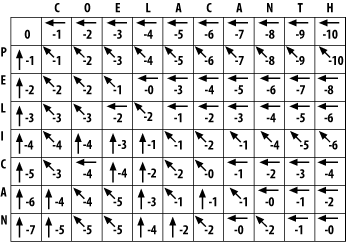
\includegraphics[width=0.65\textwidth]{images/full_matrix}
  \end{center}
\end{frame}  
   
\begin{frame}
  \frametitle{Traceback}
  \begin{center}
    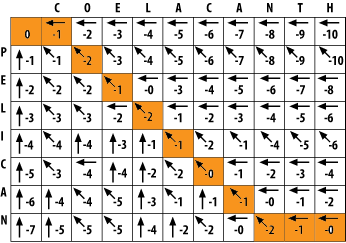
\includegraphics[width=0.65\textwidth]{images/traceback} \\
    
\includegraphics[width=0.3\textwidth]{images/traceback_sequence}         
  \end{center}
\end{frame}     

\begin{frame}
  \frametitle{Algorithms}
  \begin{itemize}
    \item<1-> Global: Needleman-Wunsch (as in example)
    \item<1-> Local: Smith-Waterman (differs from example)
    \item<2-> Biological information encapsulated \emph{only} in the scoring scheme (matches, mismatches, gaps)
    \item<3-> NW/SW are \emph{guaranteed} to find the optimal match \emph{with respect to the scoring system being used}
    \item<3-> Alignment is an approximation: no scoring scheme encapsulates biological ``truth''
    \item<3-> Any pair of sequences can be aligned: finding meaning is up to you
  \end{itemize}
\end{frame}   
  %% Advanced dynamic programming information too much for introduction
  %\include{sections/subsection_dynamicprogramming_advanced}

% BLAST in particular
\section{BLAST}
  % The BLAST Algorithm
%
% Cartoonish introduction to the BLAST algorithm

\subsection{The BLAST Algorithm}
\begin{frame}
  \frametitle{BLAST Is A Heuristic}
  \begin{itemize}
    \item<1-> BLAST does not use Needleman-Wunsch or Smith-Waterman
    \item<1-> BLAST \emph{approximates} dynamic programming methods
    \item<1-> BLAST is not guaranteed to give an optimal alignment (for chosen parameters)
    \item<2-> BLAST does not explore the complete search space
    \item<3-> BLAST uses heuristics (loosely-defined rules) to refine High-scoring Segment Pairs (HSPs)
    \item<4-> BLAST reports only ``statistically-significant'' alignments (dependent on parameters)
  \end{itemize}
\end{frame}

\begin{frame}
  \frametitle{Steps in the Algorithm}
  \begin{enumerate}
    \item Seeding
    \item Extension
    \item Evaluation
  \end{enumerate}
\end{frame}

  % BLAST seeding
%
% Basic description of the seeding component of the BLAST algorithm

\subsection{BLAST Seeding}
\begin{frame}
  \frametitle{Word Hits}
  \begin{itemize}
    \item A \emph{word hit} is a short sequence and its \emph{neighbourhood}
    \item \emph{neighbourhood}: words of same length whose aligned score is greater than or equal to a threshold value $T$
    \item Three parameters: scoring matrix, word size $W$, and $T$
  \end{itemize}
  \begin{center}
    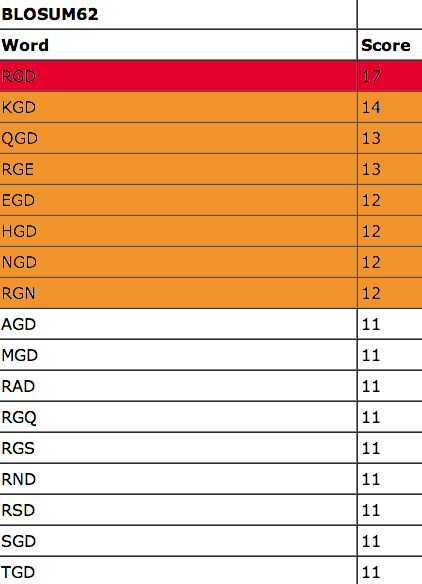
\includegraphics[width=0.3\textwidth]{images/neighbourhood} 
  \end{center}    
\end{frame}

\begin{frame}
  \frametitle{Seeding}
  \begin{itemize}
    \item BLAST assumption: significant alignments have \emph{words} in common
    \item BLAST finds word (\emph{neighbourhood}) hits in the database index
    \item Word hits are used to \textit{seed} alignments
  \end{itemize}
  \begin{center}
    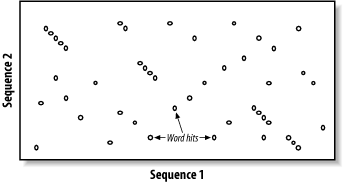
\includegraphics[width=0.5\textwidth]{images/seeding} 
  \end{center}    
\end{frame}

\begin{frame}
  \frametitle{Seeding Controls Sensitivity}
  \begin{itemize}
    \item Word size $W$ controls number of hits (smaller words $\implies$ more hits)
    \item Threshold score $T$ controls number of hits (lower threshold $\implies$ more hits)
    \item Scoring matrix controls which words match
  \end{itemize}
  \begin{center}
    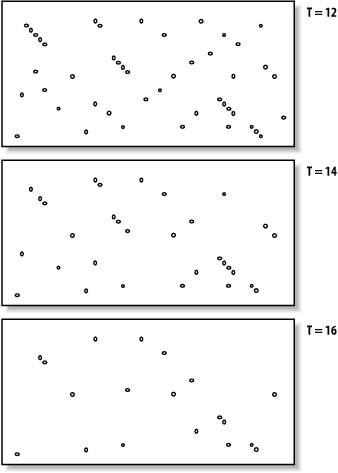
\includegraphics[width=0.25\textwidth]{images/seeding_t} 
  \end{center}    
\end{frame}

\begin{frame}
  \frametitle{The Two-Hit Algorithm}
  \begin{itemize}
    \item BLAST assumption: word hits cluster on the diagonal for significant alignments
    \item The acceptable distance $A$ between words on the diagonal is a parameter of your model
    \item Smaller distances isolate single words, and reduce search space
  \end{itemize}
  \begin{center}
    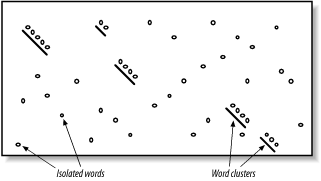
\includegraphics[width=0.5\textwidth]{images/two_hit} 
  \end{center}    
\end{frame}

  % BLAST Extension
%
% Basic description of the extension stage of the BLAST algorithm

\subsection{BLAST Extension}
\begin{frame}
  \frametitle{Extension}
  \begin{itemize}
    \item The best-scoring seeds are extended in each direction
    \item BLAST does not explore the complete search space, so a rule (heuristic) to stop extension is needed
    \item Two-stage process:
    \begin{itemize}
      \item Extend, keeping alignment score, and \emph{drop-off} score
      \item When drop-of score reaches a threshold $X$, trim alignment back to top score
    \end{itemize}
  \end{itemize}
  \begin{center}
    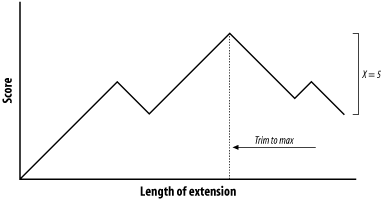
\includegraphics[width=0.5\textwidth]{images/extension} 
  \end{center}    
\end{frame}

\begin{frame}
  \frametitle{Example}
  \begin{itemize}
    \item<1-> Consider two sentences (match=+1, mismatch=-1)
    \begin{itemize}
      \item \texttt{The quick brown fox jumps over the lazy dog.}
      \item \texttt{The quiet brown cat purrs when she sees him.}
    \end{itemize}
    \item<2-> Extend to the right from the seed \texttt{T}
    \begin{itemize}
      \item \texttt{The quic}
      \item \texttt{The quie}
      \item \texttt{123 4565 <- score}
      \item \texttt{000 0001 <- drop-off score}        
    \end{itemize}
  \end{itemize}
\end{frame}

\begin{frame}
  \frametitle{Example}
  \begin{itemize}
    \item Consider two sentences (match=+1, mismatch=-1)
    \begin{itemize}
      \item \texttt{The quick brown fox jumps over the lazy dog.}
      \item \texttt{The quiet brown cat purrs when she sees him.}
    \end{itemize}
    \item Extend to drop-off threshold
    \begin{itemize}
      \item \texttt{The quick brown fox jump}
      \item \texttt{The quiet brown cat purr}
      \item \texttt{123 45654 56789 876 5654 <- score}
      \item \texttt{000 00012 10000 123 4345 <- drop-off score}        
    \end{itemize}
  \end{itemize}
\end{frame}

\begin{frame}
  \frametitle{Example}
  \begin{itemize}
    \item Consider two sentences (match=+1, mismatch=-1)
    \begin{itemize}
      \item \texttt{The quick brown fox jumps over the lazy dog.}
      \item \texttt{The quiet brown cat purrs when she sees him.}
    \end{itemize}
    \item Trim back from drop-off threshold to get optimal alignment
    \begin{itemize}
      \item \texttt{The quick brown}
      \item \texttt{The quiet brown}
      \item \texttt{123 45654 56789 <- score}
      \item \texttt{000 00012 10000 <- drop-off score}        
    \end{itemize}
  \end{itemize}
\end{frame}

\begin{frame}
  \frametitle{Notes on implementation}
  \begin{itemize}
%    \item This example represents ungapped BLAST; gapped BLAST is more similar to dynamic programming
    \item $X$ controls termination of alignment extension, but dependent on:
    \begin{itemize}
      \item substitution matrix
      \item gap opening and extension parameters
    \end{itemize}
  \end{itemize}
  \begin{center}
    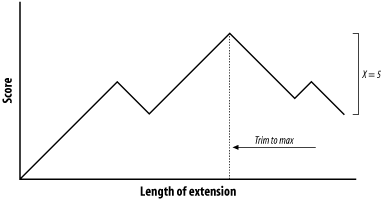
\includegraphics[width=0.5\textwidth]{images/extension} 
  \end{center}    
\end{frame}
  % BLAST Evaluation
%
% Basic outline of the extension step of the BLAST algorithm

\subsection{BLAST Evaluation}
\begin{frame}
  \frametitle{Evaluation}
  \begin{itemize}
    \item The principle is easy: use a score threshold $S$ to determine strong and weak alignments
    \begin{itemize}
      \item $S$ is monotonic with $E$, so an equivalent threshold can be calculated
    \end{itemize}
    \item Score $S$ is independent of database size and search space. $E$ values are not.
    \item Alignment consistency is also a consideration
  \end{itemize}
  \begin{center}
    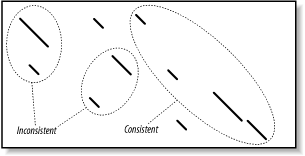
\includegraphics[width=0.5\textwidth]{images/consistency} 
  \end{center}    
\end{frame}

  %% BLAST databases too much information for introductory course
  %% BLAST Databases
%
% Introductory slides on BLAST databases

\subsection{BLAST Databases}
\begin{frame}
  \frametitle{About BLAST databases$\ldots$}
  \begin{itemize}
    \item The database used is a parameter in your BLAST search
    \item Three components:
    \begin{itemize}
      \item header file: \texttt{*.phr}, \texttt{*.nhr}
      \item sequence file: \texttt{*.psq}, \texttt{*.nsq}
      \item index file: \texttt{*.pin}, \texttt{*.nin}
    \end{itemize}
    \item The index allows for fast searching                
  \end{itemize}
\end{frame}

% BLAST statistics
\section{BLAST Statistics}
  %% Information theory section too much for introduction to biologists
  %% Information Theory
%
% Brief introduction to the bits of information theory essential for understanding BLAST

\subsection{Information Theory}
\begin{frame}
  \frametitle{Bits of Information}
  \begin{itemize}
    \item<1-> The amount of information in a thing (e.g. a message, or picture) can be measured in \emph{bits}, and represented as $H$ (entropy)
    \item<1-> One bit = one "yes/no" or "1/0" answer
    \item<2-> The information associated with a probability $p$ can be represented in bits: \\
              $H(p) = -\text{log}_2(p)$
    \item<2-> For a series of $n$ probabilities $\{p_i,$\ldots$, p_n\}$ we have: \\
              $H = -\sum^{n}_{i} p_i \text{log}_2 (p_i)$
  \end{itemize}
\end{frame}

\begin{frame}
  \frametitle{Information in Random Alphabets}
  \begin{itemize}
    \item DNA and protein alphabets have multiple symbols, so have different entropies (are not equally informative)
    \item Assuming random sequences (no symbol bias):
    \begin{itemize}
      \item For a coin, $p(H) = p(T) = 0.5 \implies H(coin) = 1\text{bit}$
      \item For DNA, $p(A) = p(C) = p(G) = p(T) = 0.25 \implies H(\text{DNA}) = 2\text{bits}$       
      \item For protein, $p(A) = p(C) = $\ldots$ = 0.05 \implies H(\text{protein}) = 4.32\text{bits}$
    \end{itemize}
    \item Twice as much information in protein than DNA alphabet
  \end{itemize}
\end{frame}

\begin{frame}
  \frametitle{Information in Biased Alphabets}
  \begin{itemize}
    \item Deviation from random sequence reduces entropy
    \begin{itemize}
      \item For DNA, $p(A) = p(C) = p(G) = p(T) = 0.25 \implies H(\text{DNA}) = 2\text{bits}$       
      \item For DNA: $p(A) = 0.4; p(C) = 0.3; p(G) = 0.2; p(T) = 0.1 \implies H(\text{DNA}) = 1.85\text{bits}$       
    \end{itemize}
    \item Biological sequences/databases deviate from randomness
  \end{itemize}
\end{frame}
  
\begin{frame}
  \frametitle{Log-odds Scores}
  \begin{itemize}
    \item<1-> How often does a symbol substitution occur, compared to random expectation?
    \item<1-> If $p(\text{Met}) = 0.01$, $p(\text{Leu}) = 0.1$, we would expect a Met-Leu substitution with frequency $p(\text{Met})p(\text{Leu}) = 0.001$
    \item<2-> Observe Met-Leu substitution with frequency $q(\text{Met-Leu}) = 0.002$
    \item<2-> Odds ratio is $\frac{q(\text{Met-Leu})}{p(\text{Met})p(\text{Leu})} = 2$
    \item<3-> Log odds ratio is $\text{log}_2(\frac{q(\text{Met-Leu})}{p(\text{Met})p(\text{Leu})}) = 1\text{bit}$
  \end{itemize}
\end{frame}  
  % Substitution matrices
%
% A basic introduction to BLAST substitution matrices

\subsection{Substitution Matrices}
\begin{frame}
  \frametitle{Log-odds Matrices}
  \begin{itemize}
    \item Substitution matrices are a model of evolution, represented by log-odds matrices
    \begin{itemize}
      \item Positive numbers indicate likely substitutions/similarity
      \item Negative numbers indicate unlikely substitutions/dissimilarity
    \end{itemize}
  \end{itemize}
  \begin{center}
   BLOSUM62 \\
   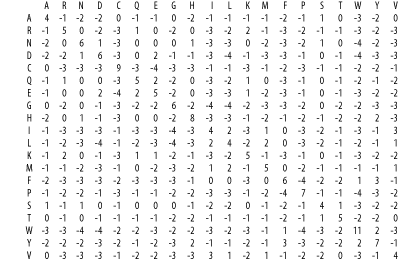
\includegraphics[width=0.5\textwidth]{images/blosum62} 
 \end{center}         
\end{frame} 

\begin{frame}
  \frametitle{Choice of Matrix}
  \begin{itemize}
    \item Substitution matrix determines the raw alignment score $S$
    \begin{itemize}
      \item $S$ is the sum of pairwise scores in an alignment
    \end{itemize}
    \item For proteins:
    \begin{itemize}
      \item \texttt{BLOSUM45 BLOSUM50 BLOSUM62 BLOSUM80 BLOSUM90}
      \item \texttt{PAM30 PAM70 PAM250}
    \end{itemize}
    \item BLOSUM matrices empirically defined from multiple sequence alignments of $\geq n\%$ identity, for \texttt{BLOSUMn}
    \item For nucleotides: `matrix' defined by match/mismatch (reward/penalty) parameters
  \end{itemize}
\end{frame} 
 
  %% Detail of target frequencies etc too much for introduction to biologists
  %% Substitution Matrices Advanced

\subsection{Substitution Matrices (advanced)}
\begin{frame}
  \frametitle{Target Frequencies}
  \begin{itemize}
    \item Target frequencies represent the underlying evolutionary model implicit in the substitution matrix
    \item Each substitution matrix has a scaling factor $\lambda$, estimated from symbol frequency
    \item $\lambda$ is used to calculate a \emph{normalised score} for the alignment, $\lambda S$
    \item In modern BLAST, $\lambda$ is also dependent on the query and subject sequence composition
  \end{itemize}
\end{frame}   

\begin{frame}
  \frametitle{Substitution Matrices}
  \framesubtitle{matrix relative entropy}
  \begin{itemize}
    \item Matrix \emph{expected score} $E$ is the sum of raw scores weighted by frequency of occurrence (should be negative)
    \begin{equation}
      E = \sum^{20}_{i=1}\sum_{j=1}^{i} p_i p_j S_{ij}
    \end{equation}
    \item Matrix \emph{relative entropy} $H$ is the average number of bits per position in an alignment generated from that matrix.
    \begin{equation}
      H = \sum^{20}_{i=1}\sum_{j=1}^{i} q_{ij} \lambda S_{ij}
    \end{equation}
  \end{itemize}
\end{frame}  
  % Karlin-Altschul Equation
%
% Basic introduction to the Karlin-Altschul equation.

\subsection{The Karlin-Altschul Equation}
\begin{frame}
  \frametitle{Definition}
  \begin{itemize}
    \item The Karlin-Altschul equation
    \begin{equation*}
      E = k m n e^{-\lambda S}
    \end{equation*}
    \item Symbols:
    \begin{itemize}
      \item $k$: minor constant, adjusts for correlation between alignments
      \item $m$: number of letters in query sequence
      \item $n$: number of letters in the database
      \item $\lambda$: scoring matrix scaling factor
      \item $S$: raw alignment score
    \end{itemize}
  \end{itemize}
\end{frame} 

\begin{frame}
  \frametitle{Interpretation}
  \begin{itemize}
    \item The Karlin-Altschul equation
    \begin{equation*}
      E = k m n e^{-\lambda S}
    \end{equation*}
    \item $E$ is the number of alignments with a similar score expected by chance when querying a database of that size and symbol frequency, where the letters in the database are randomly-ordered
    \item Small changes in score $S$ can produce large changes in $E$
    \item Biological sequence databases are not random!
  \end{itemize}
\end{frame} 
  %% Detail of equation assumptions etc too much for introduction to biologists
  %% The Karlin-Altschul equation (advanced)

\subsection{The Karlin-Altschul Equation (advanced)}
\begin{frame}
  \frametitle{Assumptions}
  \begin{itemize}
    \item The Karlin-Altschul equation
    \begin{equation*}
      E = k m n e^{-\lambda S}
    \end{equation*}
    \item Assumptions:
    \begin{itemize}
      \item A positive score must be possible
      \item The scoring matrix \emph{expected score} must be negative
      \item Sequences are infinitely long
      \item Alignments do not contain gaps
      \item Sequence symbols (bases, residues) are independent and identically-distributed
    \end{itemize}
  \end{itemize}
\end{frame}  
  
% Using BLAST   
\section{Using BLAST}
  % Which BLAST tool should I use?
%
% Short introduction to some of the range of BLAST tools available

\subsection{Which BLAST tool should I use?}
\begin{frame}
  \frametitle{Multiple BLAST \textit{tools}}
  \begin{itemize}
    \item BLASTN \textit{vs} MEGABLAST \textit{vs} TBLASTX \textit{vs} ...?
    \item Korf \textit{et al.} (2003) BLAST is really good for theory part, \\
             but practical examples dated due to changes with BLAST+
  \end{itemize}
  \begin{center}
    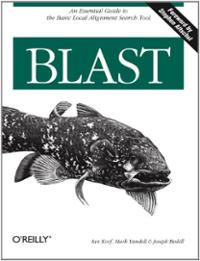
\includegraphics[width=.2\textwidth]{images/korf_book}
  \end{center}
\end{frame}

\begin{frame}
  \frametitle{Multiple \textit{ways} to run BLAST}
  \begin{itemize}
    \item BLAST+ at the command line (today)
    \item Via a script or programming language
    \item Via a graphical tool like BioEdit, CLCbio, Blast2GO
    \item Via the NCBI website
    \item Via a genome consortium website
    \item Via a Galaxy web server
    \item etc
    \item Offers flexibility \textit{but} different settings/options/versions
  \end{itemize}
\end{frame}

\begin{frame}
  \frametitle{Multiple \textit{places} to run BLAST}
  \begin{itemize}
    \item On the NCBI servers, e.g. via website or tool
    \item On 3rd party servers, e.g. via websites
    \item On your own computer
    \item On our Linux cluster
  \end{itemize}
\end{frame}

\begin{frame}
  \frametitle{Core BLAST tools: Query sequences \textit{vs} Database}
  \begin{itemize}
    \item Nucleotide \textit{vs} Nucleotide:
    \begin{itemize}
      \item \texttt{blastn} (covering blastn, megablast, dc-megablast)
    \end{itemize}
    \item Translated nucleotide \textit{vs} Protein:
    \begin{itemize}
      \item \texttt{blastx}
    \end{itemize}
    \item Protein \textit{vs} Translated nucleotide:
    \begin{itemize}
      \item \texttt{tblastn}
    \end{itemize}
    \item Protein \textit{vs} Protein:
    \begin{itemize}
      \item \texttt{blastp}, \texttt{psiblast}, \texttt{phiblast}, \texttt{deltablast}
    \end{itemize}
  \end{itemize}
  See \url{http://blast.ncbi.nlm.nih.gov/} for a reminder ;)
\end{frame}

  % BLAST at the command-line
%
% Basic examples of BLAST at the command line

\subsection{Running BLAST+ at the command line}
% [fragile] frames must end with \end{frame} directly following a newline, or they break!
\begin{frame}[fragile]
  \frametitle{The BLAST tools have built in help}
\begin{lstlisting}[language=sh]
$ blastp -h
USAGE
  blastp [-h] [-help] [-import_search_strategy filename]
    [-export_search_strategy filename] [-task task_name] [-db database_name]
    [-dbsize num_letters] [-gilist filename] [-seqidlist filename]
    [-negative_gilist filename] [-entrez_query entrez_query]
    [-db_soft_mask filtering_algorithm] [-db_hard_mask filtering_algorithm]
    [-subject subject_input_file] [-subject_loc range] [-query input_file]
    [-out output_file] [-evalue evalue] [-word_size int_value]
    [-gapopen open_penalty] [-gapextend extend_penalty]
    [-xdrop_ungap float_value] [-xdrop_gap float_value]
    [-xdrop_gap_final float_value] [-searchsp int_value] [-max_hsps int_value]
    [-sum_statistics] [-seg SEG_options] [-soft_masking soft_masking]
    [-matrix matrix_name] [-threshold float_value] [-culling_limit int_value]
    ...
    [-max_target_seqs num_sequences] [-num_threads int_value] [-ungapped]
    [-remote] [-comp_based_stats compo] [-use_sw_tback] [-version]

DESCRIPTION
   Protein-Protein BLAST 2.2.29+

Use '-help' to print detailed descriptions of command line arguments
\end{lstlisting}
\end{frame}

% [fragile] frames must end with \end{frame} directly following a newline, or they break!
\begin{frame}[fragile]
  \frametitle{Minimal example of BLAST+ at the command line}
\begin{lstlisting}[language=sh]
$ blastp -query my_input.fasta -db my_database -out my_output.txt
\end{lstlisting}
  \begin{itemize}
    \item Replace \texttt{blastp} with the appropriate tool, e.g. \texttt{blastn}
    \item Replace \texttt{my\_input.fasta} with your actual filename
    \item Replace \texttt{my\_database} with your actual database, e.g. \text{nr}
    \item Replace \texttt{my\_output.txt} with your desired output filename
    \item Best to avoid spaces in your folder and filenames!
  \end{itemize}
  e.g.
\begin{lstlisting}[language=sh]
$ blastp -query query.fasta -db dbA -out my_output.txt
\end{lstlisting}
\end{frame}

  % Controlling BLAST output format

\subsection{Controlling BLAST output}
% [fragile] frames must end with \end{frame} directly following a newline, or they break!
\begin{frame}[fragile]
  % Verbally note that the NCBI BLAST website lets you pick the
  % format at the end. Can do something similar with the special
  % BLAST archive format, but would be a distraction?
  \frametitle{Setting the BLAST+ output format}
\begin{lstlisting}[language=sh]
$ blastp -help
USAGE
...

 *** Formatting options
 -outfmt <String>
   alignment view options:
     0 = pairwise,
     1 = query-anchored showing identities,
     2 = query-anchored no identities,
     3 = flat query-anchored, show identities,
     4 = flat query-anchored, no identities,
     5 = XML Blast output,
     6 = tabular,
     7 = tabular with comment lines,
     8 = Text ASN.1,
     9 = Binary ASN.1,
    10 = Comma-separated values,
    11 = BLAST archive format (ASN.1)

   ...
   Default = `0'
...
\end{lstlisting}
\end{frame}

% [fragile] frames must end with \end{frame} directly following a newline, or they break!
\begin{frame}[fragile]
  \frametitle{Setting the BLAST+ output format}
  Default is plain text pairwise alignments, for humans:
\begin{lstlisting}[language=sh]
$ blastp -query query.fasta -db dbA -out my_output.txt
...
\end{lstlisting}
  XML output can be useful (e.g. for BLAST2GO):
\begin{lstlisting}[language=sh]
$ blastp -query query.fasta -db dbA -out my_output.xml -outfmt 5
...
\end{lstlisting}
  Tabular output is easiest to filter, sort, etc:
\begin{lstlisting}[language=sh]
$ blastp -query query.fasta -db dbA -out my_output.tab -outfmt 6
...
\end{lstlisting}
\end{frame}

  % Setting BLAST parameters
%
% Basic introduction to setting common BLAST parameters

\begin{frame}[fragile]
  \frametitle{Setting the e-value threshold}
  Check the built in help:
\begin{lstlisting}[language=]
$ blastp -help
USAGE
...
 -evalue <Real>
   Expectation value (E) threshold for saving hits
   Default = `10'
...
\end{lstlisting}
  Example using $0.0001$ or $1 \times 10^{-5}$ in scientific notation (\texttt{1e-5})
\begin{lstlisting}[language=sh]
$ blastp -query query.fasta -db dbA -out my_output.txt -evalue 1e-5
...
\end{lstlisting}
\end{frame}

  %% TODO: Interpreting BLAST output
  %\include{sections/subsection_blastinterp}     

\begin{frame}
  \frametitle{In Conclusion}
  \begin{itemize}
    \item Every BLAST search is an experiment
    \item Badly-designed searches can give you bad results
    \item Knowing how BLAST works helps improve search design
    \item BLAST results still require inspection and interpretation
  \end{itemize}
\end{frame}     
    
% etc
\end{document}
